~\begin{figure}[h!]
	~\begin{subfigure}[b]{\linewidth}
		\centering
		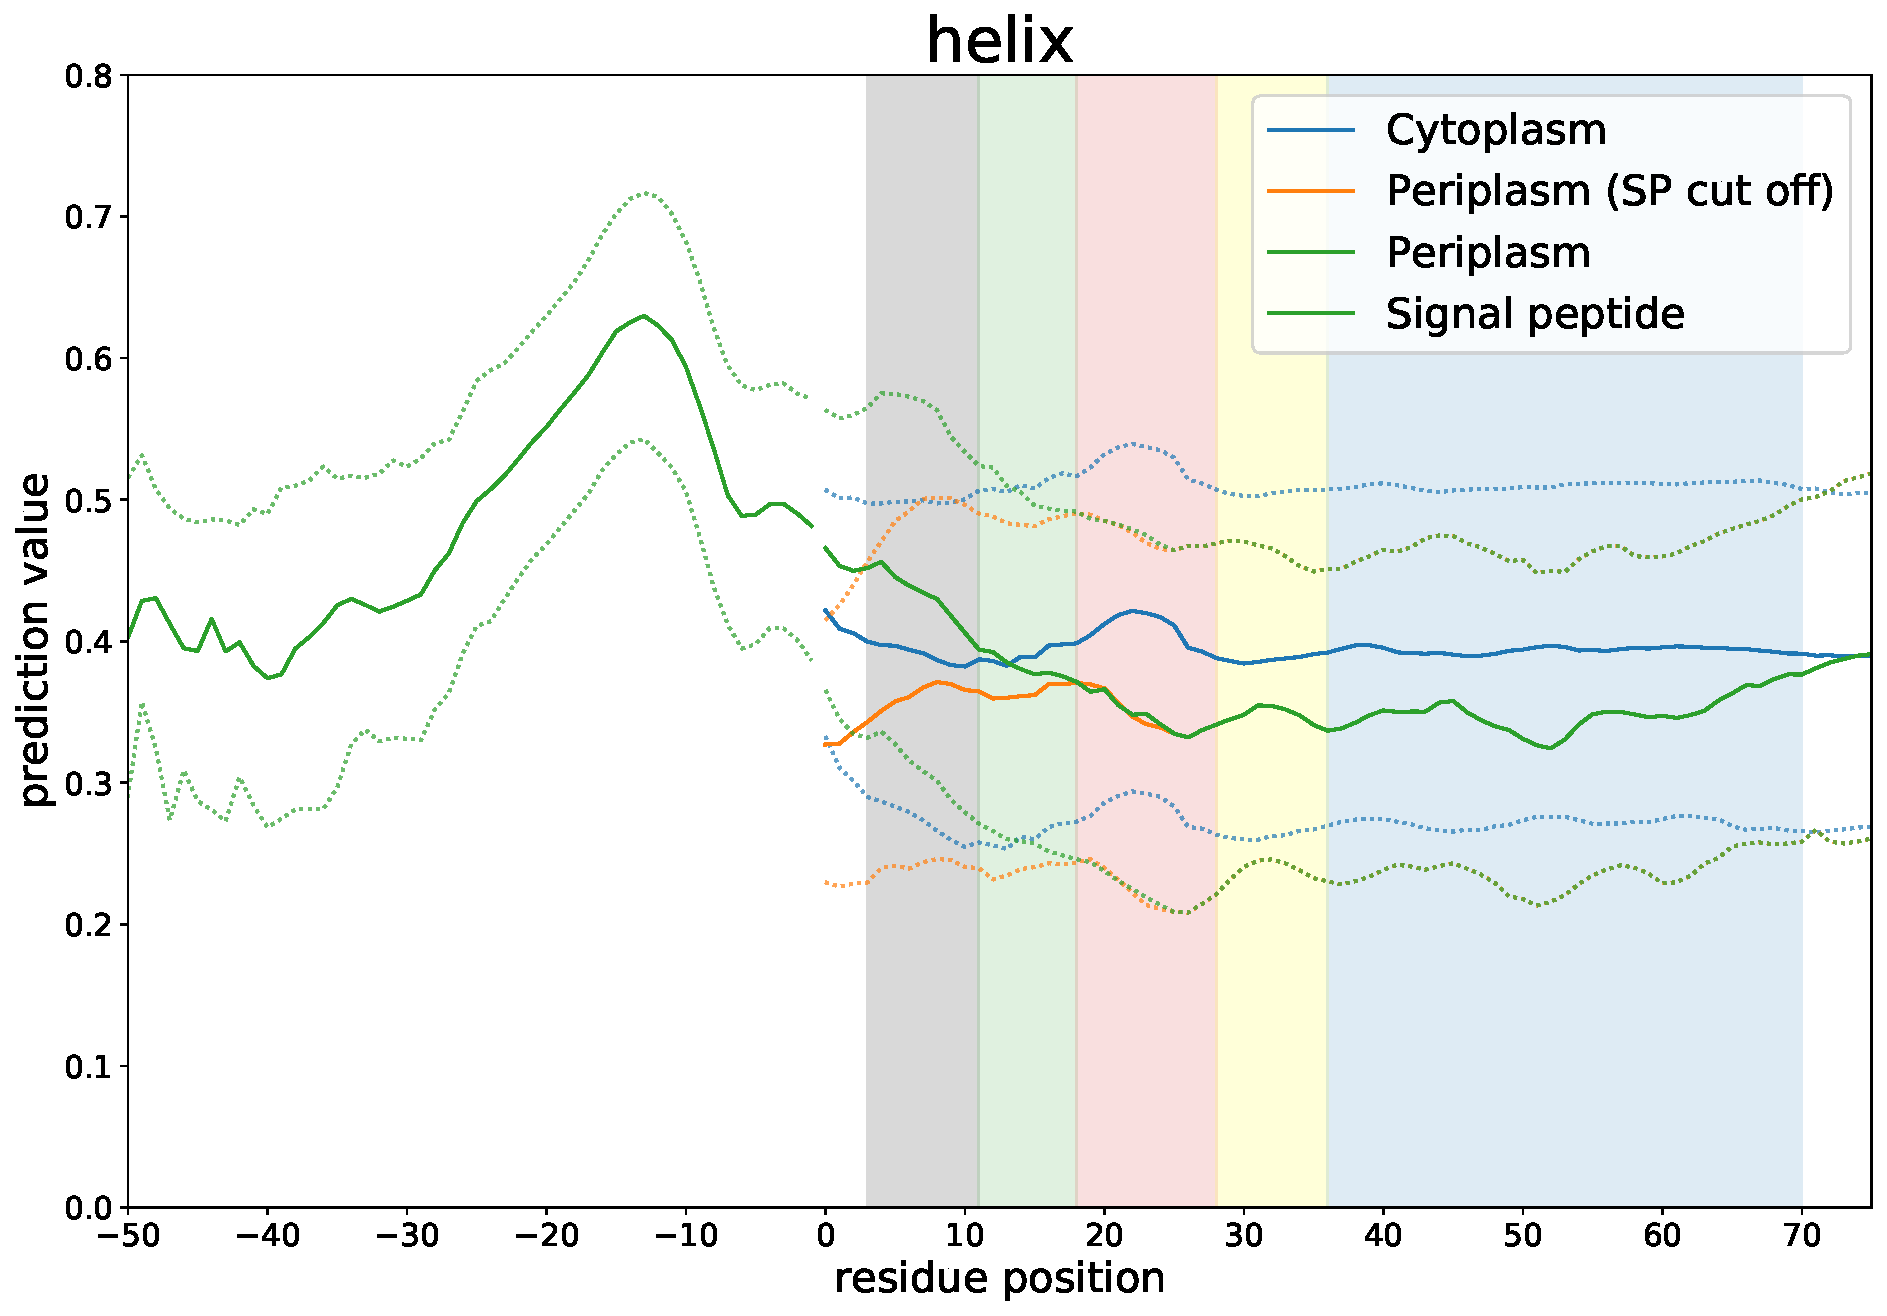
\includegraphics[width=\linewidth, height=0.46\textheight, keepaspectratio]{./results/general_comparison/local_comparison/img/local_helix.pdf}
		\label{fig:local_helix}
	~\end{subfigure}
	\newline
	~\begin{subfigure}[b]{\linewidth}
		\centering
		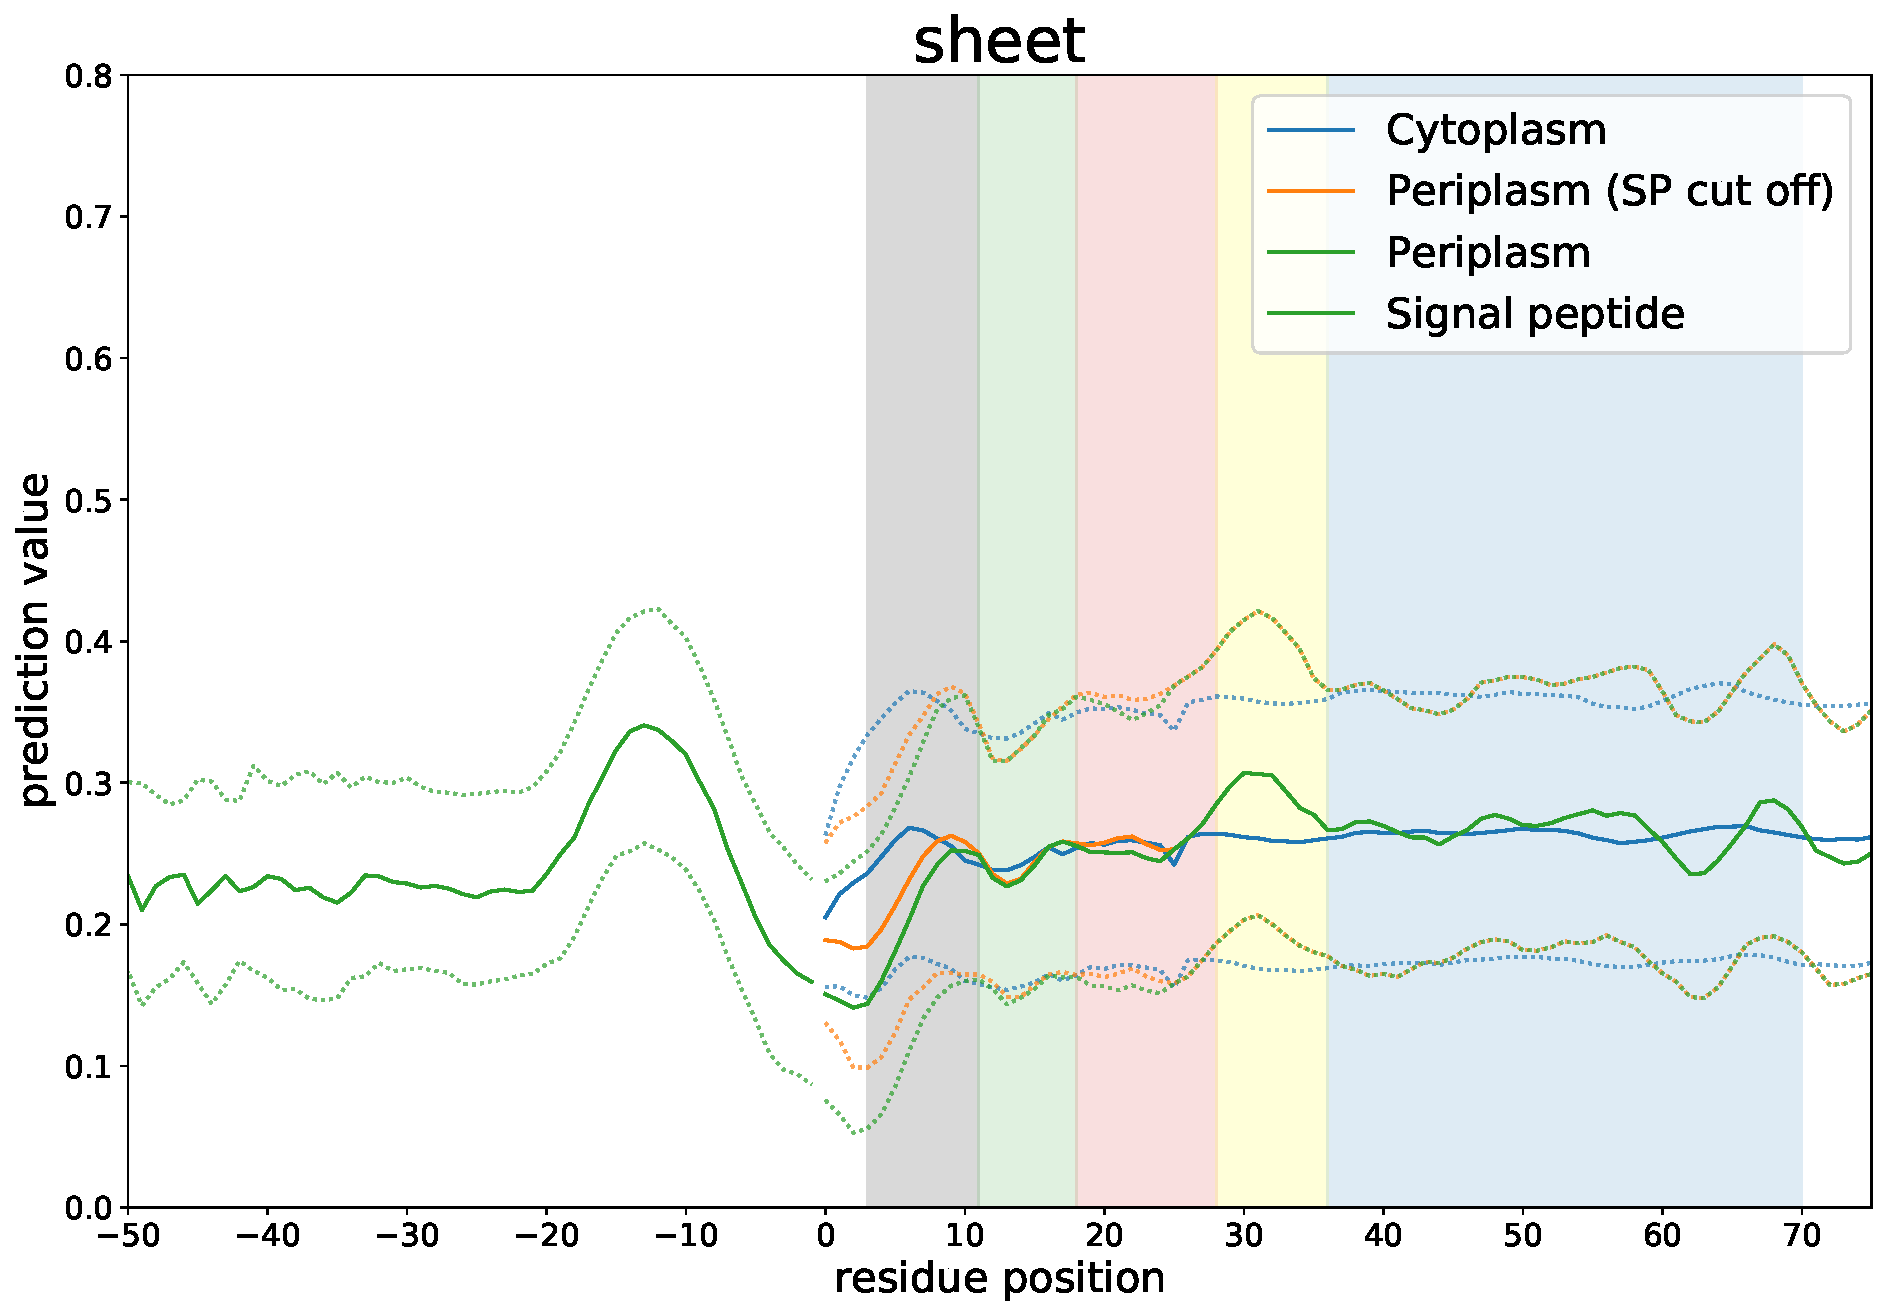
\includegraphics[width=\linewidth, height=0.46\textheight, keepaspectratio]{./results/general_comparison/local_comparison/img/local_sheet.pdf}
		\label{fig:local_sheet}
	~\end{subfigure}
~\end{figure}

~\begin{figure}[h!]
	\ContinuedFloat
	~\begin{subfigure}[b]{\linewidth}
		\centering
		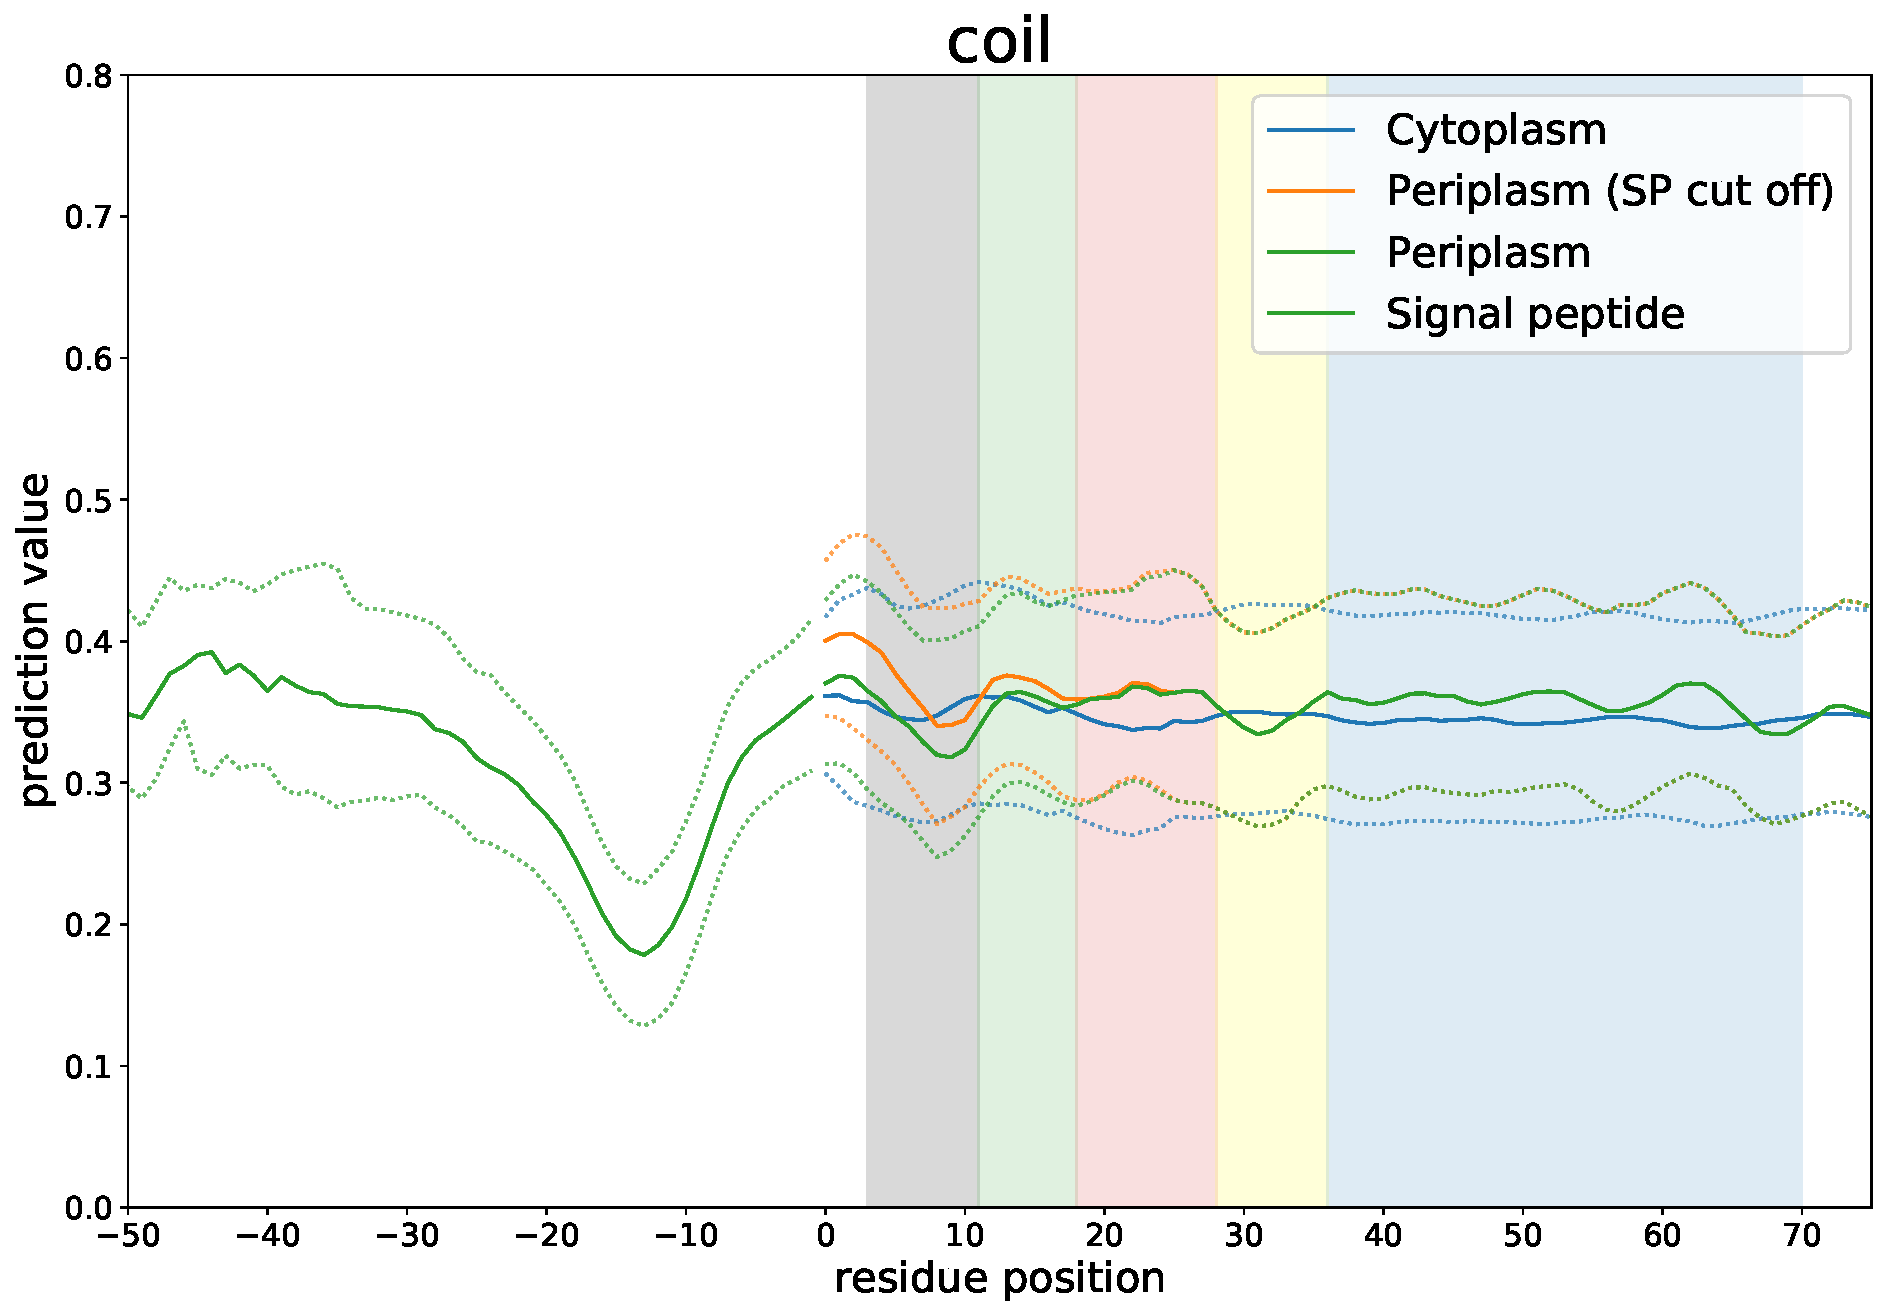
\includegraphics[width=\linewidth, height=0.46\textheight, keepaspectratio ]{./results/general_comparison/local_comparison/img/local_coil.pdf}
		\label{fig:local_coil}
	~\end{subfigure}
	\newline
	~\begin{subfigure}[b]{\linewidth}
		\centering
		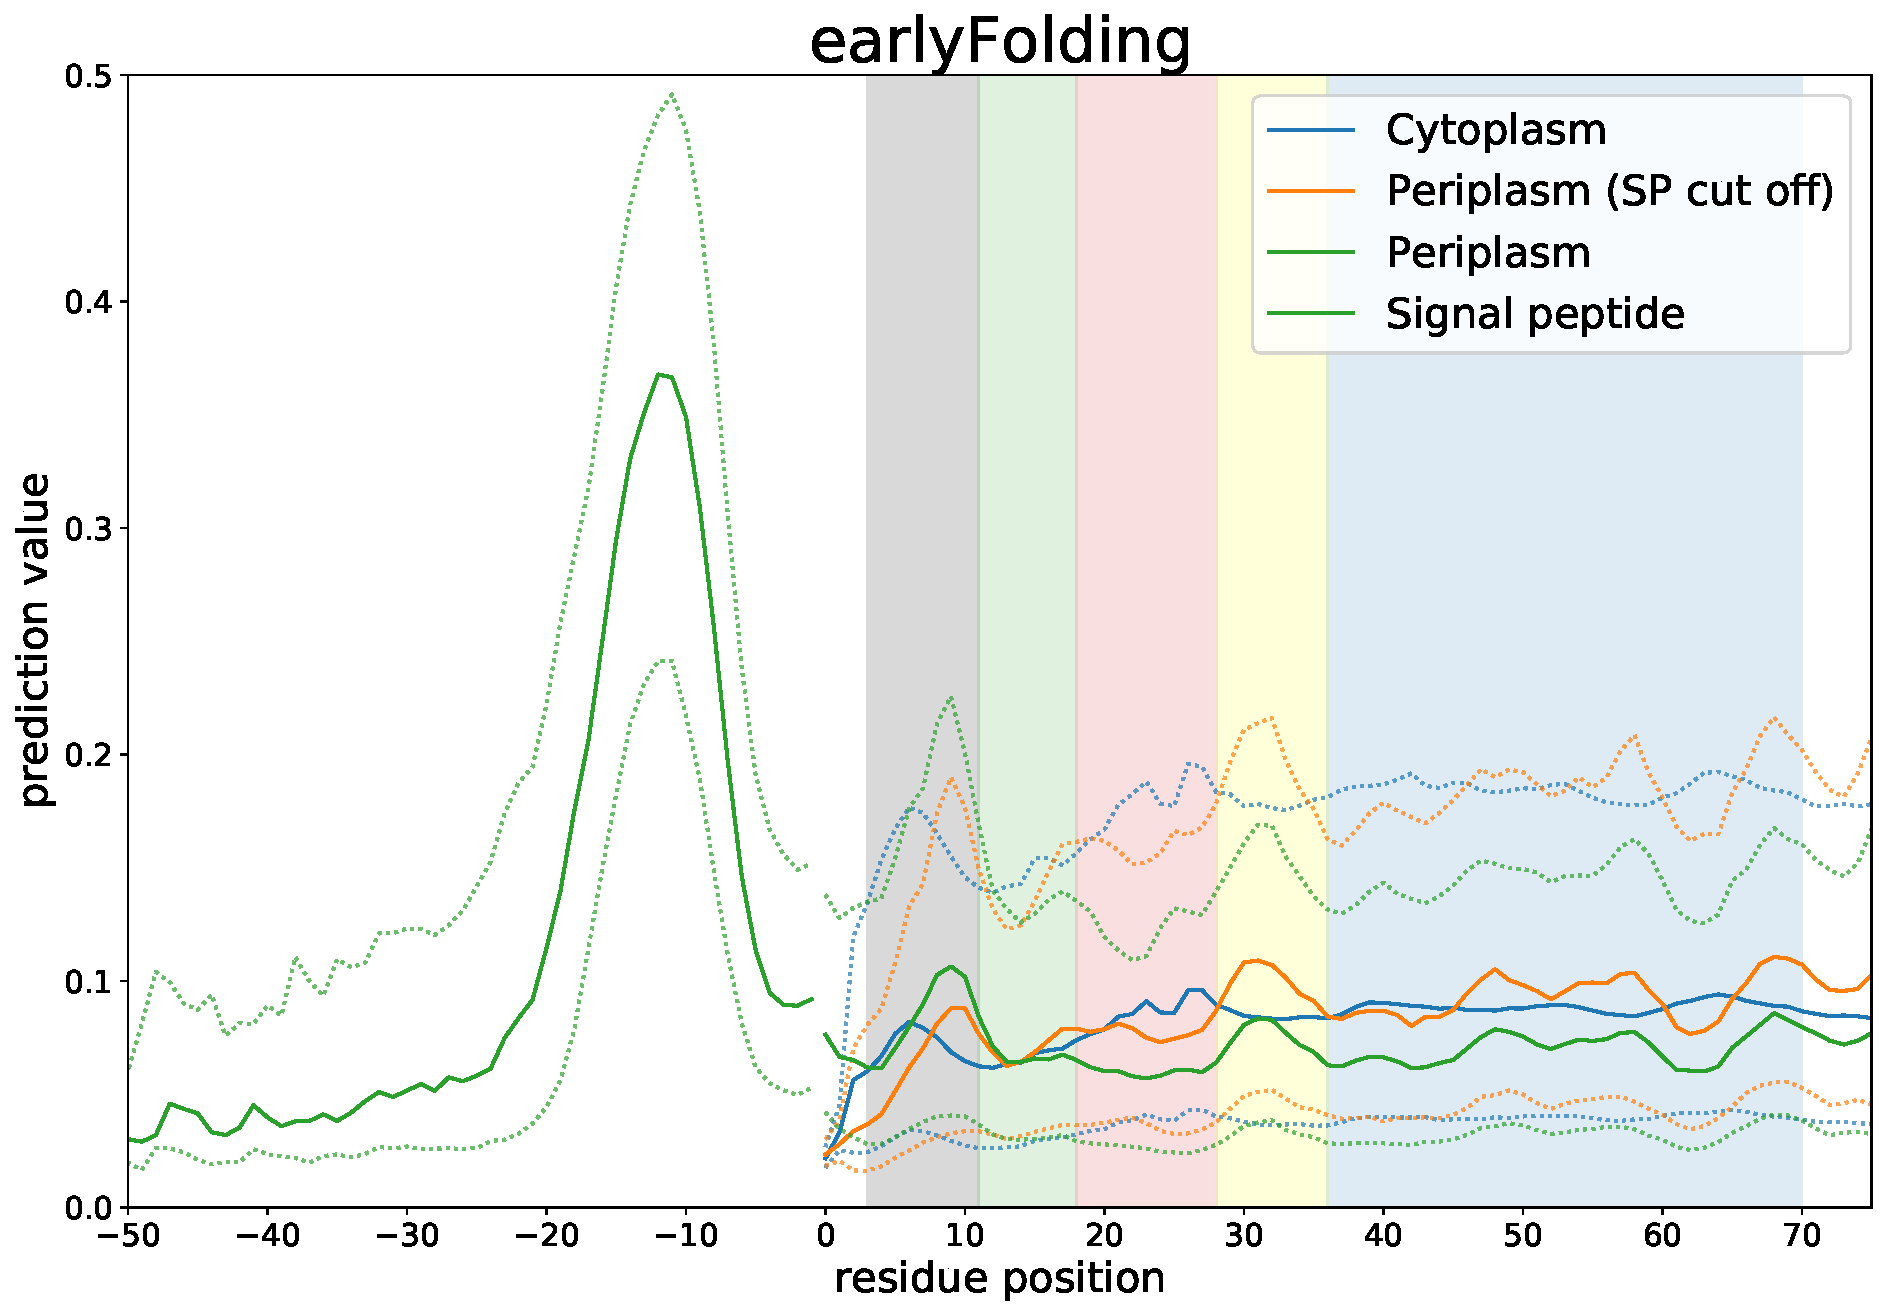
\includegraphics[width=\linewidth, height=0.46\textheight, keepaspectratio ]{./results/general_comparison/local_comparison/img/local_earlyFolding.pdf}
		\label{fig:local_earlyfolding}
	~\end{subfigure}
~\end{figure}


~\begin{figure}[h!]
	\ContinuedFloat
	~\begin{subfigure}[b]{\linewidth}
		\centering
		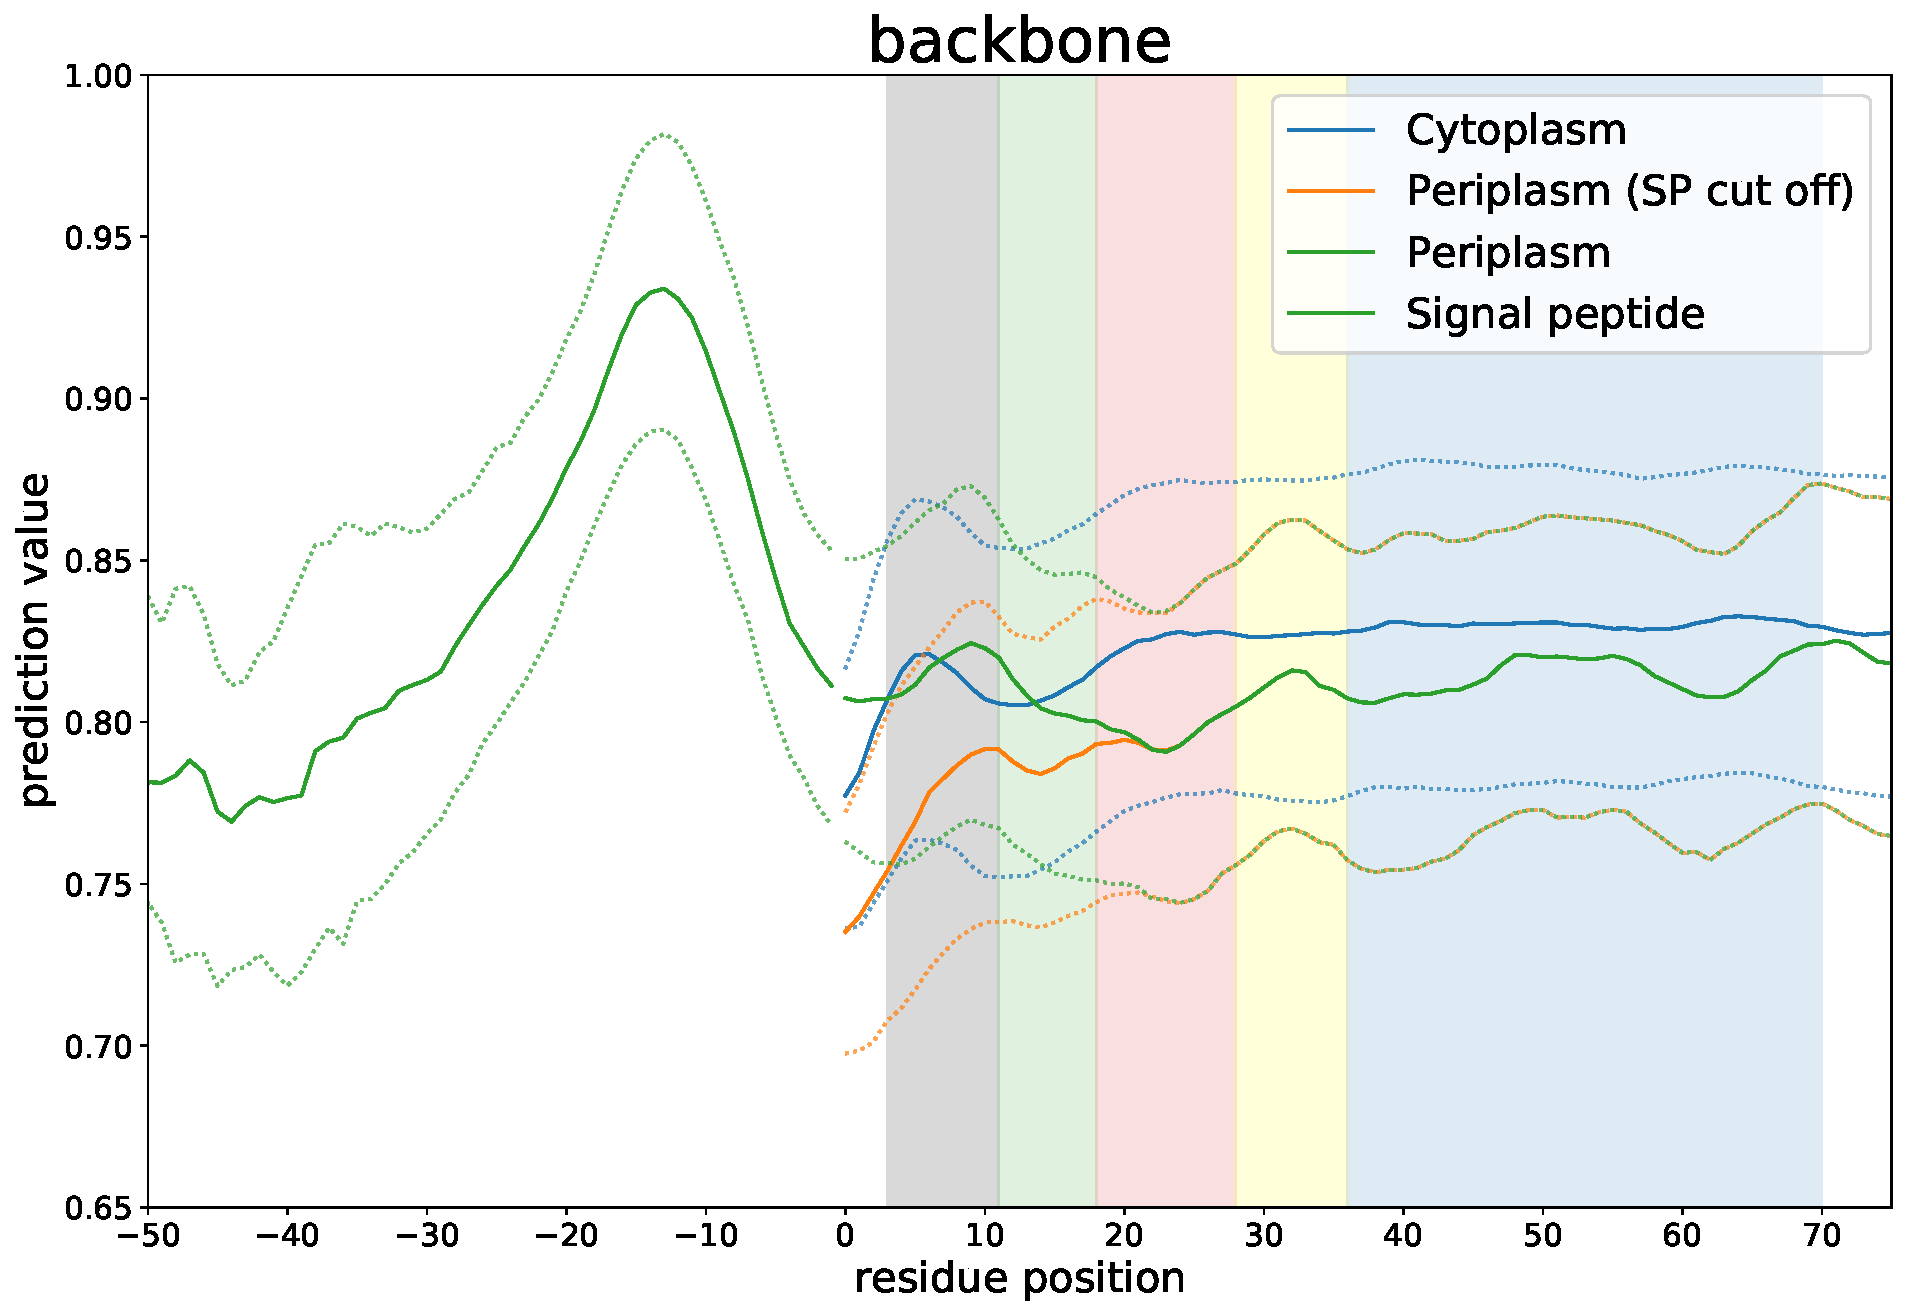
\includegraphics[width=\linewidth, height=0.37\textheight, keepaspectratio ]{./results/general_comparison/local_comparison/img/local_backbone.pdf}
		\label{fig:local_sheet}
	~\end{subfigure}
	\newline
	~\begin{subfigure}[b]{\linewidth}
		\centering
		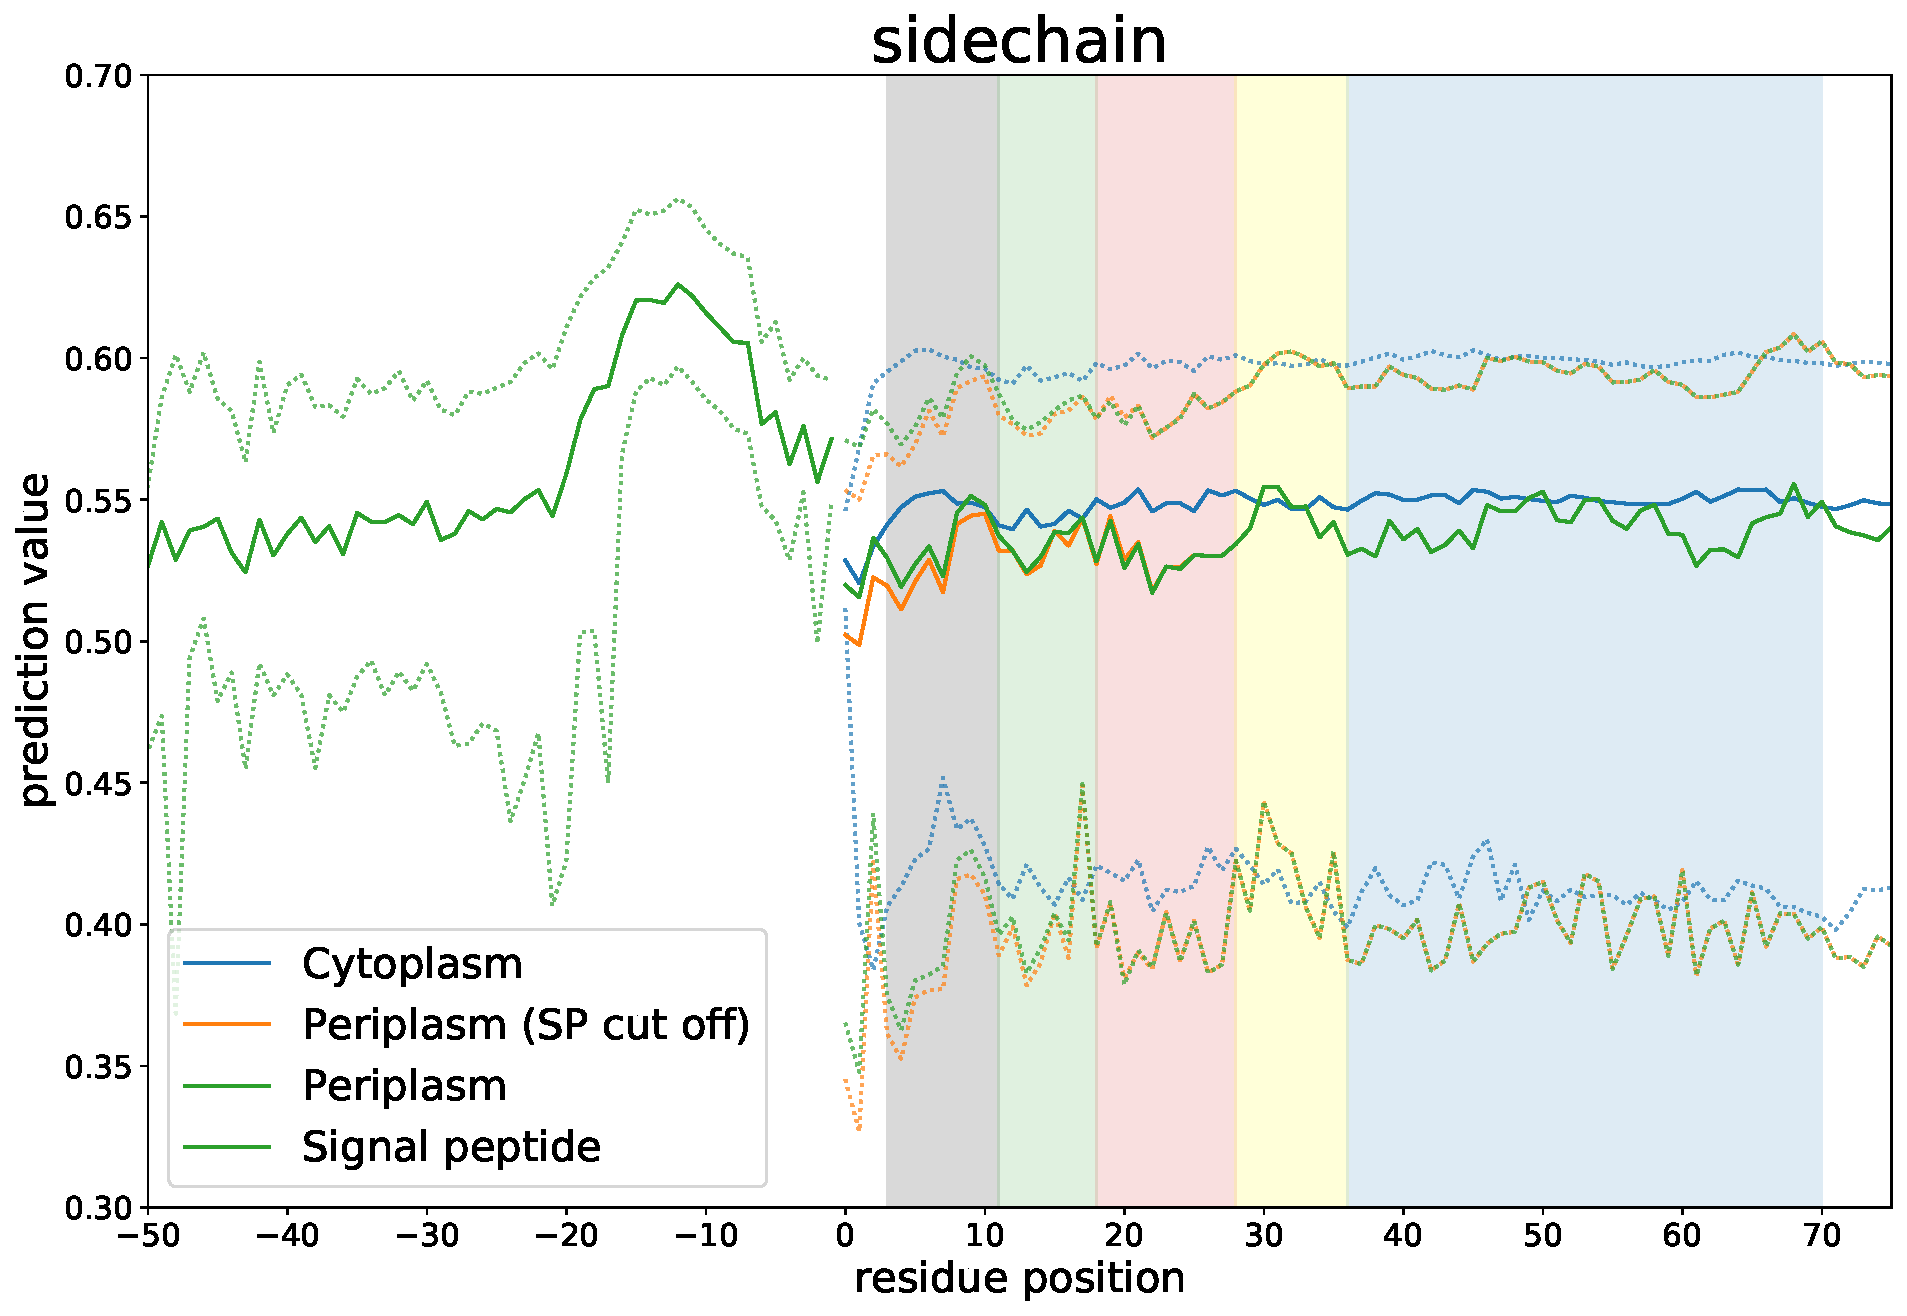
\includegraphics[width=\linewidth, height=0.37\textheight, keepaspectratio ]{./results/general_comparison/local_comparison/img/local_sidechain.pdf}
		\label{fig:local_coil}
	~\end{subfigure}
	\caption{
		\textbf{Propensity toward helix formation.}
		For each residue position, the median, first and third quartile were calculated.	
		Medians are shown by full colored lines,
		the quartiles by the dotted lines.
		Signal peptides are annotated with negative positions 
		so that the mature domains are aligned with the cytoplasmic protein.
		DynaMine only uses local sequence information to predict biophysical features.
		Therefore, the effect of the signal peptide is only observed on the graph until residue position 25.
		For later residue positions, the periplasm curve with signal peptide cut off (orange) and periplasm curve including the signal peptide (green) completely overlap.
		EFoldMine predictions (early folding) on the other hand can show distant effects on early folding of the signal peptide.
		\textbf{Signal Peptide}:residue -50 -- 0,
		\textbf{Grey region}:residue 3 -- 11,
		\textbf{Green region}:residue 11 -- 18,
		\textbf{Red region}:residue 18 -- 28,
		\textbf{Yellow region}:residue 28 -- 36,
		\textbf{Blue region}:residue 36 -- 70.
	}
	\label{fig:local_features}
~\end{figure}

